\chapter{บันทึกการปฎิบัติงานในบริษัท}
\label{chapter:atmosphere}
\section{บรรยากาศของสถานที่}
บริษัท Nextzy Technologies เป็นบริษัทตั้งอยู่ใจกลางเมืองอยู่ใกล้ทั้ง รถไฟ MRT BTS Airport link และเรือคลองแสนแสบ
อยู่ตึกอโศกทาวเวอร์ ชั้น 7 ภายในบริษัทมีห้องประชุมที่เอื้ออำนวยทั้งการประชุม การพรีเซ้นหรือจัดสอนหรือแบ่งปันเรื่องราว 
และเอื้ออำนวยแก่การพักผ่อน และบริษัทยังมีโต๊ะพลูและบอร์ดเกมเพื่อให้พนักงานคลายเครียดและเพิ่มความสัมพันธ์กันภายในบริษัท
\section{บรรยากาศภายในบริษัท}
ภายในบริษัทให้ความยืดหยุ่นแก่การทำงาน เข้างานก่อน 11:00น เลิกงานหลังเวลาที่ตนเข้างาน เพิ่มอีก 9 ชั่วโมงและมีการประชุมบริษัทประจำเดือนเพื่อแจ้งเกี่ยวกับความคืบหน้าภายในบริษัท 
และภายในบริษัทจะเซอร์ไพร์วันเกิดพนักงานจัดโดยพนักงานกันเอง 
\\
\begin{figure}[!htbp]
      \centering
      \subfigure[ประชุมบริษัทประจำเดือน]{
            \label{Fig:meeting}
            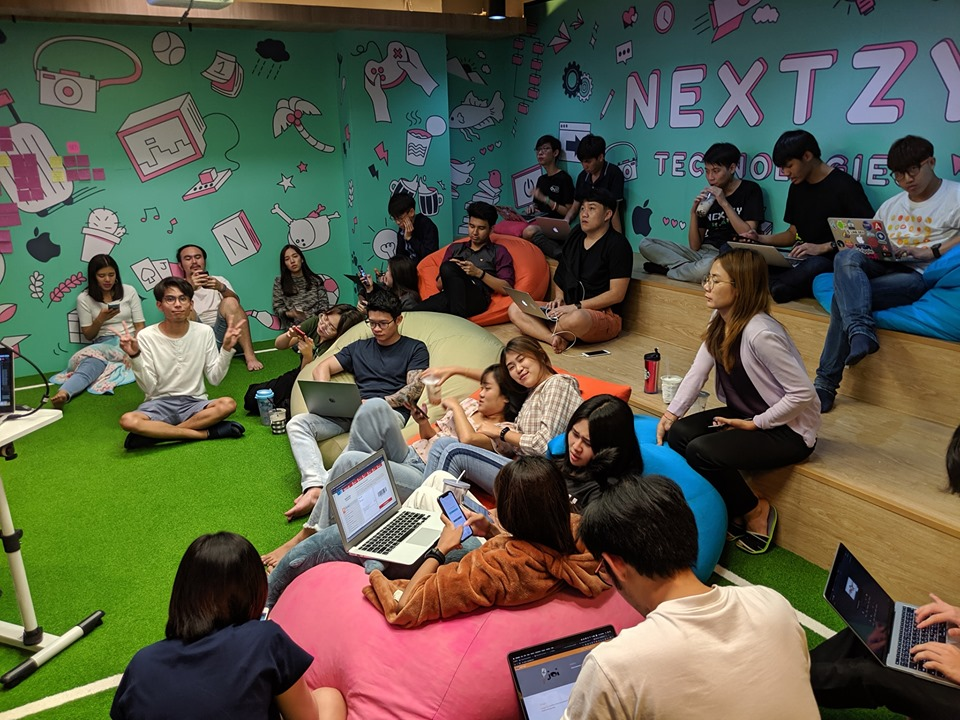
\includegraphics[width=0.7\linewidth]{meeting}
      }
     
\end{figure}
\begin{figure}[!htbp]
      \centering
      \subfigure[บรรยากาศตอนนั่งทำงาน]{
            \label{Fig:work}
            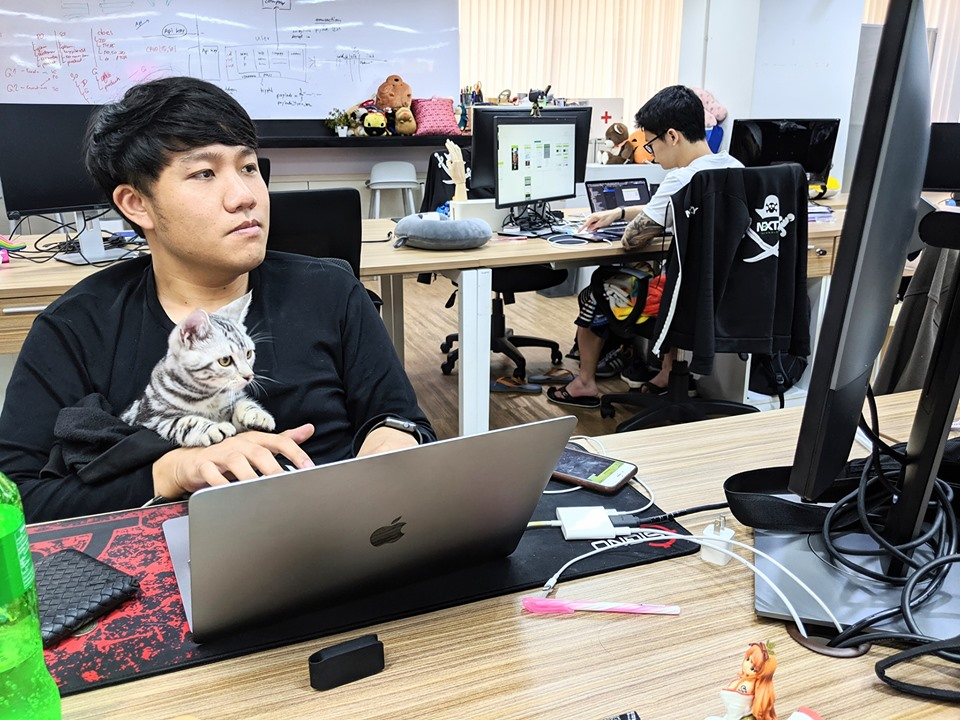
\includegraphics[width=0.8\linewidth]{work}
      }
      \subfigure[เซอร์ไพร์เค้กวันเกิดพนักงานด้วยของโปรด]{
            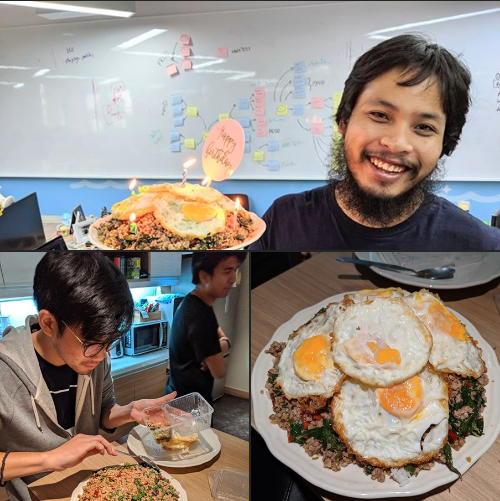
\includegraphics[width=0.7\linewidth]{hbd}
            \label{Fig:hbd}
      }
      \caption{บรรยากาศภายในบริษัท}
\end{figure}
\newpage
\section{กิจกรรมหลังเลิกงาน}
 ภายในบริษัทมีนโยบายกระชับมิตรกันภายในบริษัท เช่น ดูหนังกันทั้งบริษัทโดยทางบริษัทออกค่าใช้จ่ายให้ หรือปาร์ตี้ประจำปี ที่สาขาจากเชียงใหม่จะลงมาร่วมปาร์ตี้ด้วย
\begin{figure}[!htbp]
      \centering
	\subfigure[ไปดูหนังทั้งบริษัท]{
            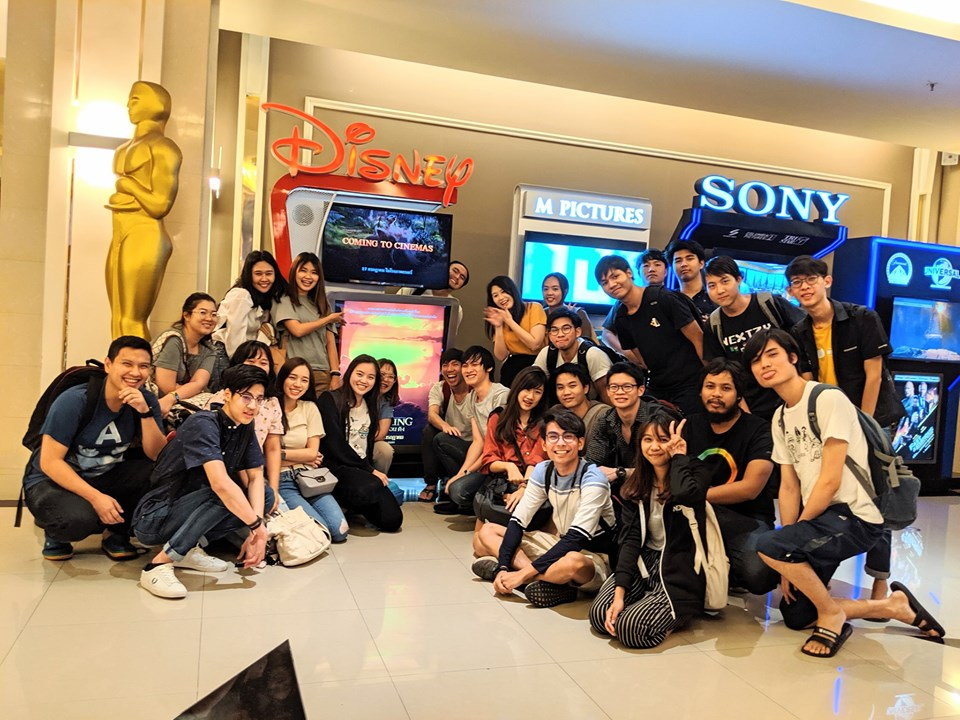
\includegraphics[width=0.48\linewidth]{movie}
            \label{Fig:movie}
      }
      \subfigure[ปาร์ตี้บริษัทประจำปี]{
            \label{Fig:party}
            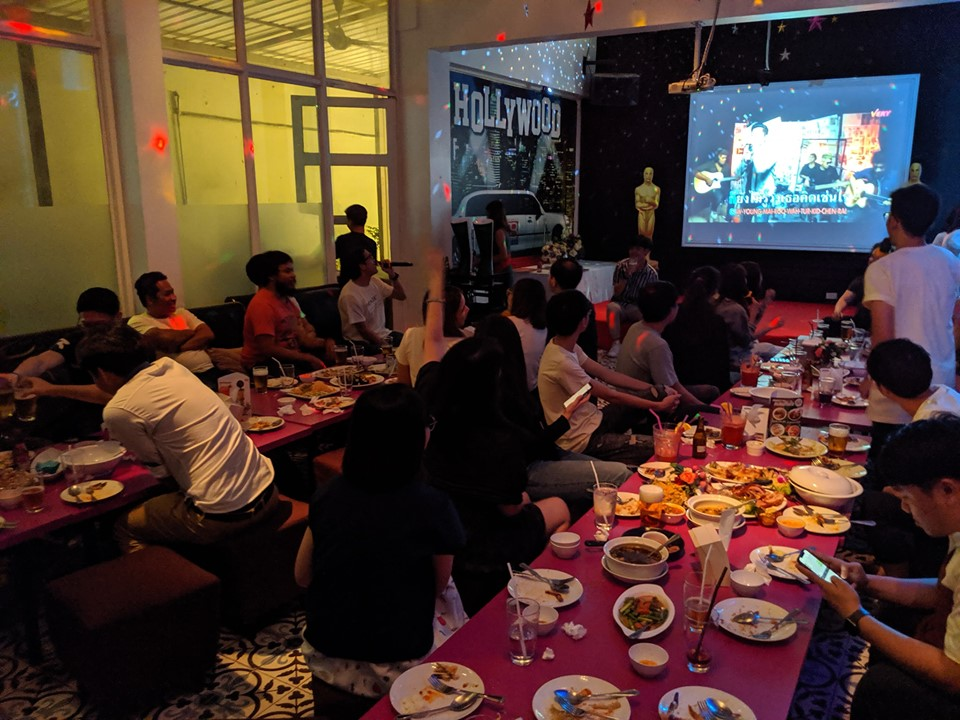
\includegraphics[width=0.48\linewidth]{party}
      }
      \subfigure[นัดดูงาน Appleภายในบริษัท]{
            \label{Fig:apple}
            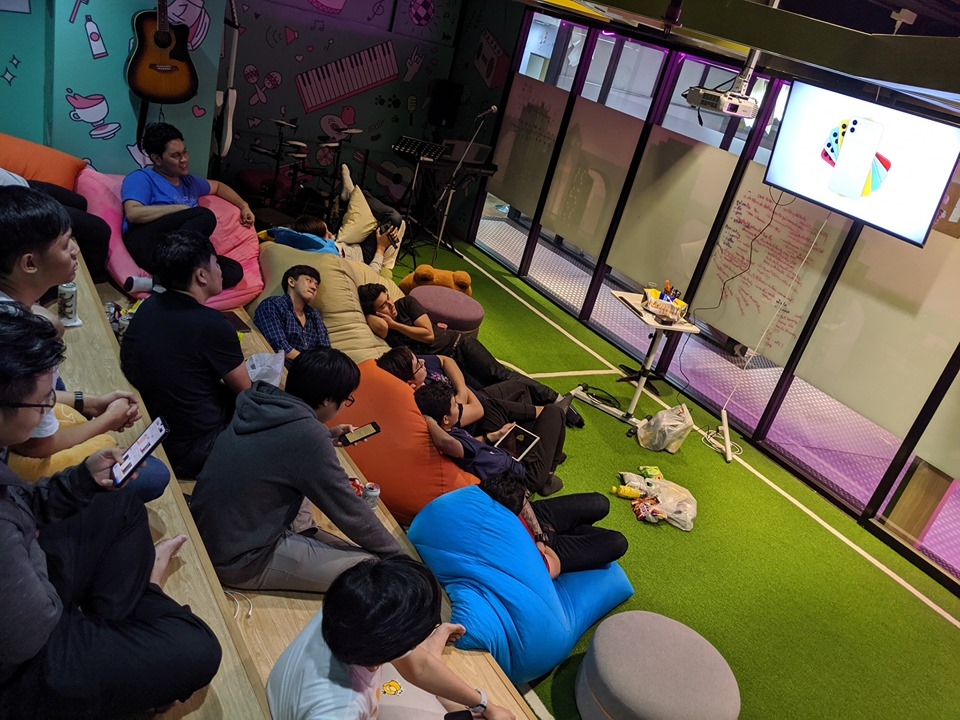
\includegraphics[width=0.48\linewidth]{apple}
      }
      \subfigure[เล่นบอร์ดเกมหลังเลิกงาน]{
            \label{Fig:game}
            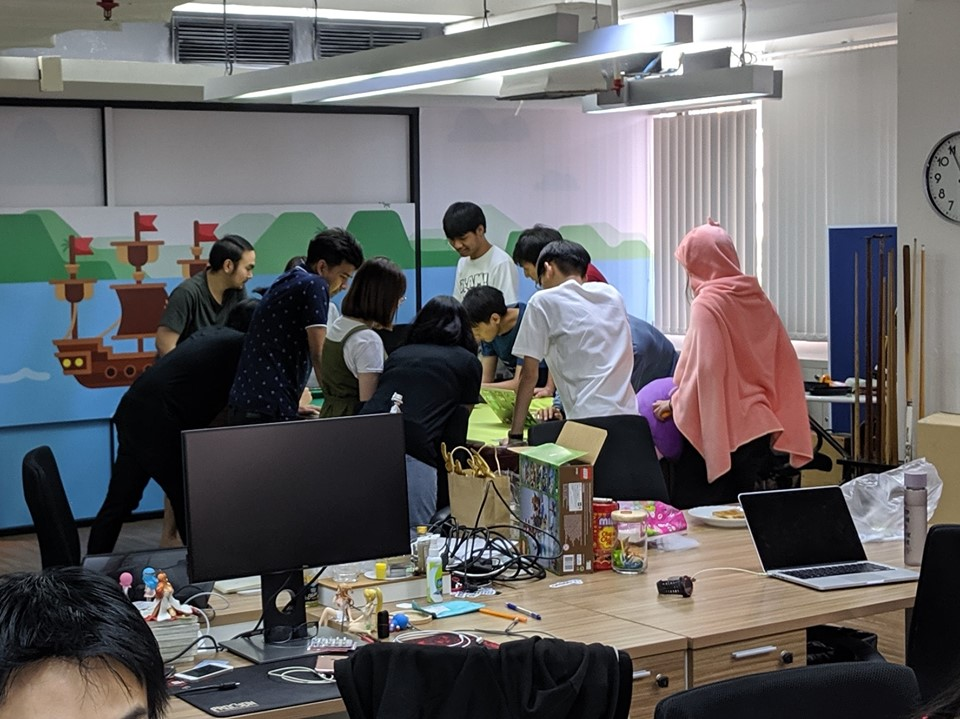
\includegraphics[width=0.48\linewidth]{game}
      }
      \caption{กิจกรรมหลังเลิกงาน}
\end{figure}
\section{อบรม Mastering Web Performance Optimization}
Skooldio ได้จัดอบรม  Web Performance Optimization โดย Warat Wongmaneekit 
ที่เป็น Google Developers Expert in Web Technologies (GDE) วันที่ 15 กันยายน พ.ศ.2562 และ ทางบริษัทเห็นว่ามีเนื้อหาอบรม
มีประโยชน์ ต่อหลายโปรเจค จึงส่งพนักงงานไปอบรม 2 คน (นักศึกษาและพนักงาน)
\begin{figure}[!htbp]
	\centering
	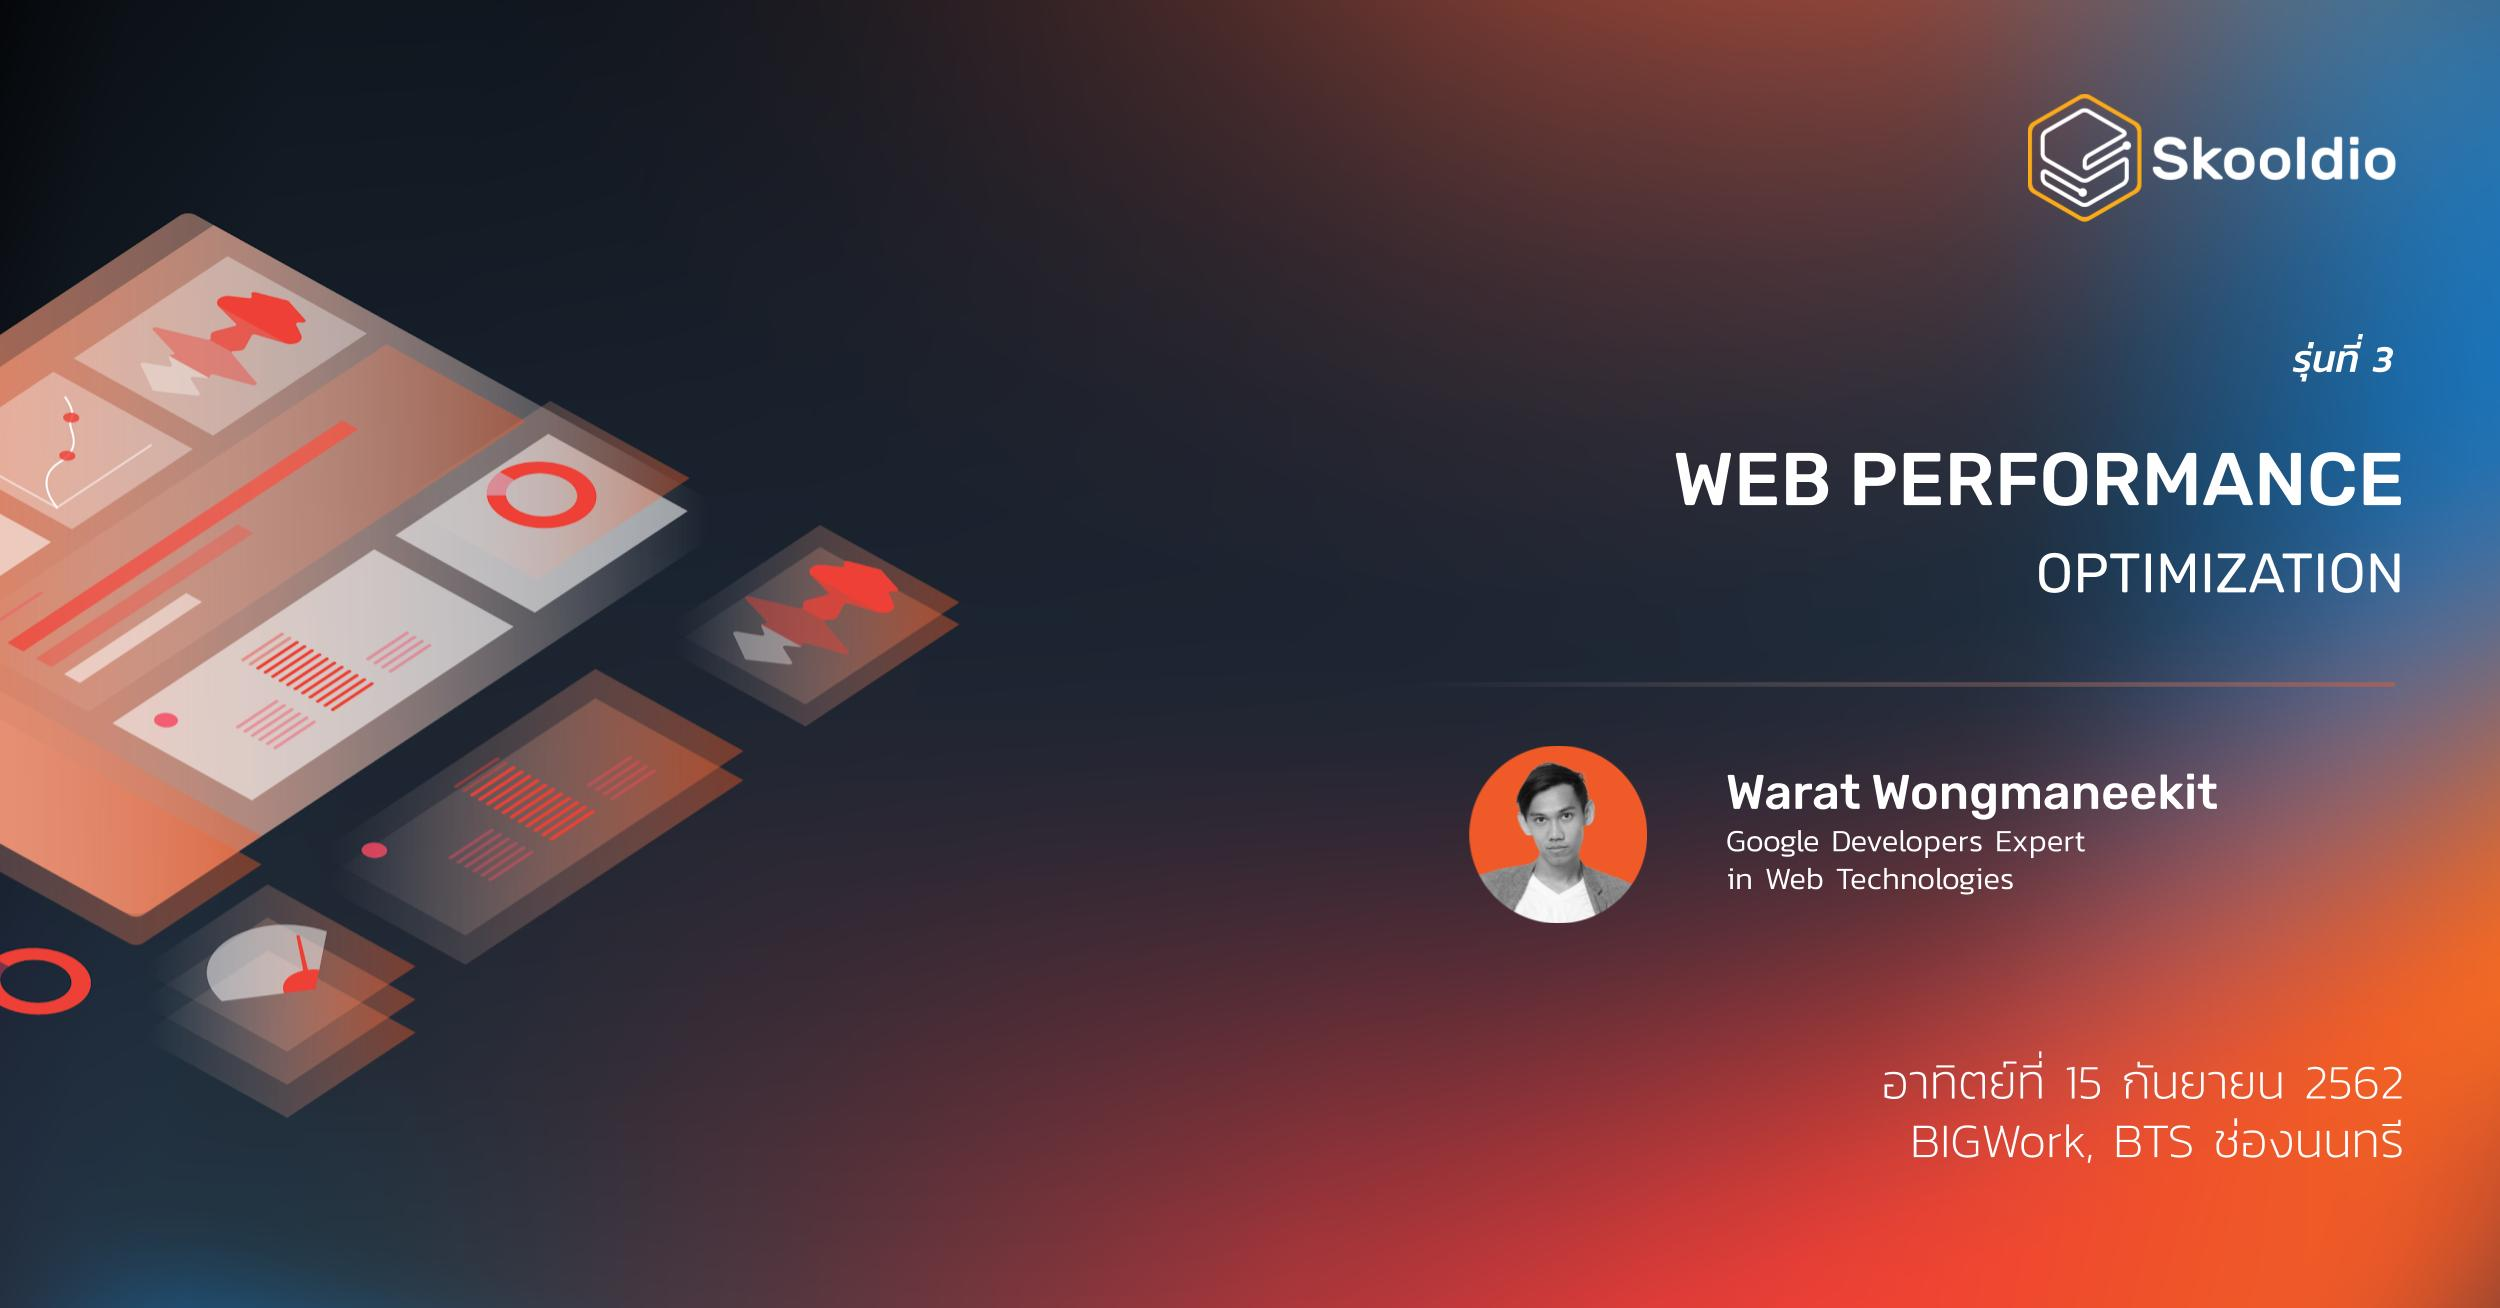
\includegraphics[width=0.75\linewidth]{WebOpt3}
	\caption{Poster Mastering Web Performance Optimization}
	\label{Fig:WebPerformance}
\end{figure}
\newpage
\section{เขียนบทความให้ความรู้ด้านเว็บ ใน Blog ของบริษัท }
ทางบริษัทมีนโยบายให้นักศึกษาฝึกงานต้องเขียน เกี่ยวกับงานด้านที่ตนทำใน Blog ของบริษัท อย่างน้อย 1 เรือง
ซึ่งนักศึกษาเองได้เขียนบทความไปถึง 3 เรื่องดังนี้
 \subsection{สร้าง Circle Spinner Menu ด้วย React และ Styled Components}
 \begin{figure}[!htbp]
	\centering
	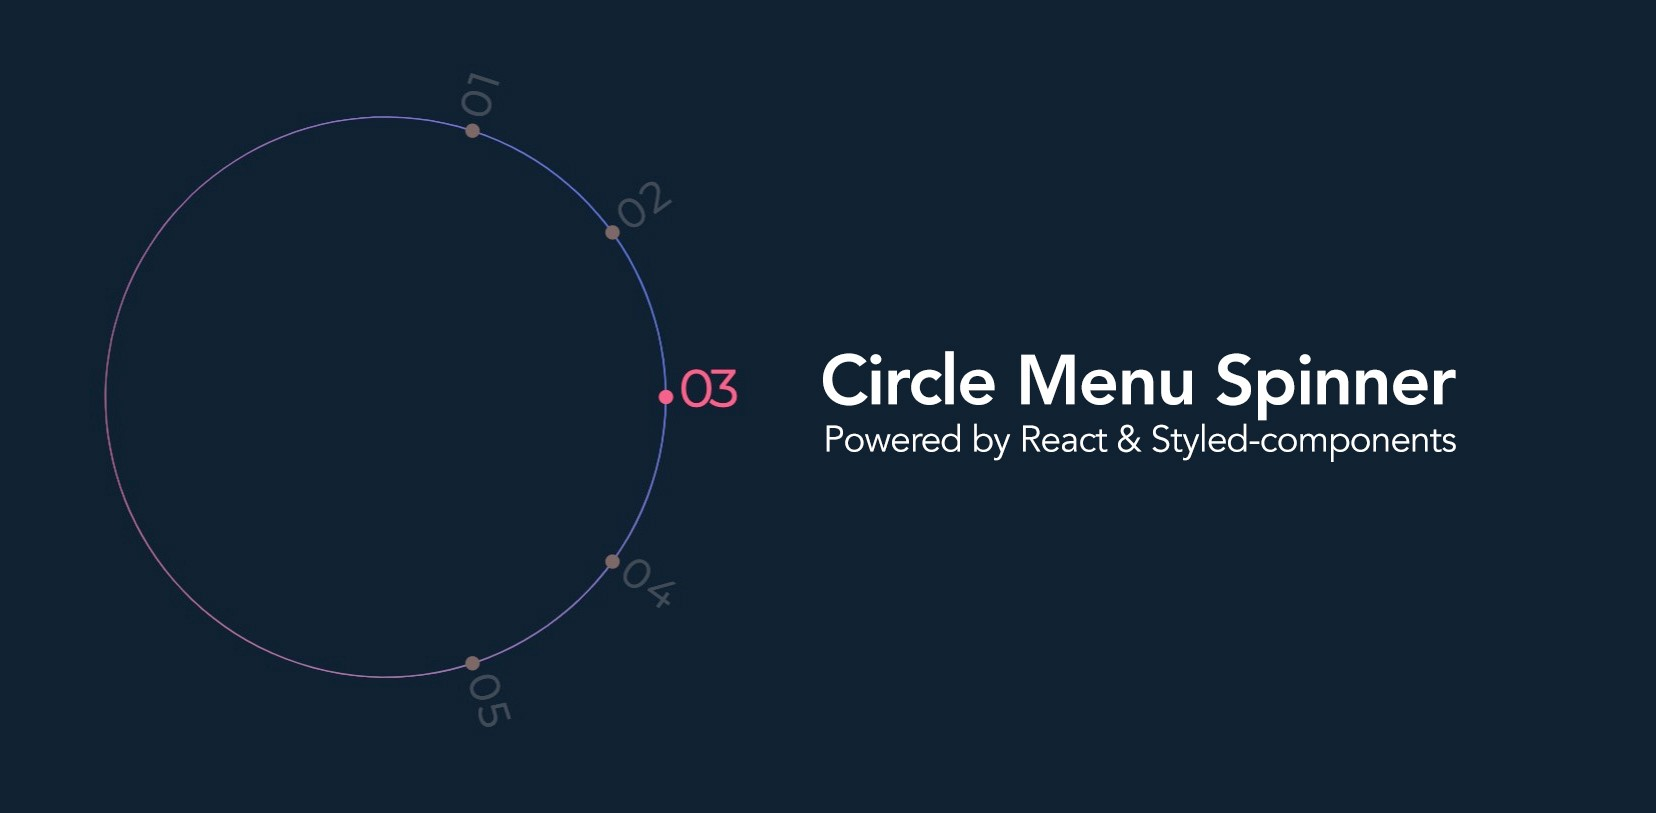
\includegraphics[width=0.8\linewidth]{blog-1}
	\caption{Circle Spinner Menu}
	\label{Fig:WebPerformance}
\end{figure}
\newpage
 \subsection{มาTerminal Customize ให้เท่ขึ้น 300\% ด้วย Oh My Zsh}
 \begin{figure}[!htbp]
	\centering
	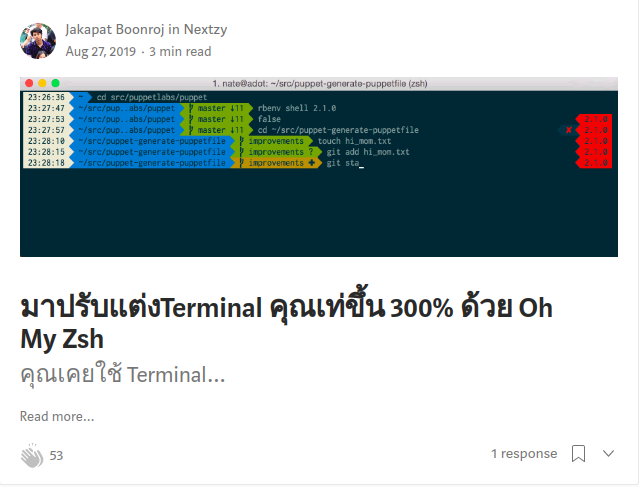
\includegraphics[width=0.8\linewidth]{blog-2}
	\caption{Terminal Customize}
	\label{Fig:WebPerformance}
\end{figure}
 \subsection{Skeleton Screen พริบตาที่ไม่ควรมองข้าม}
 \begin{figure}[!htbp]
	\centering
	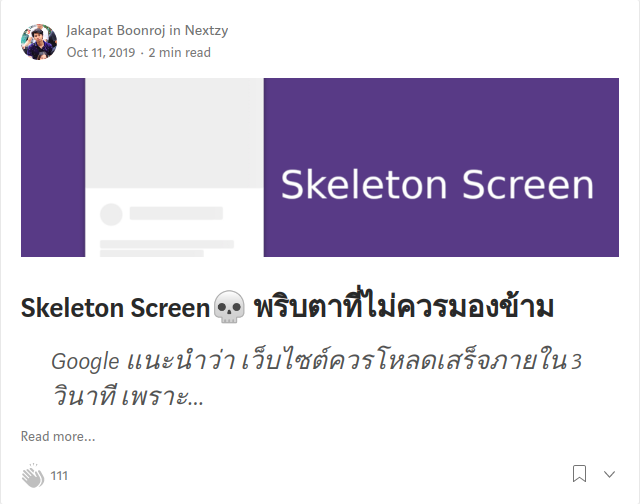
\includegraphics[width=0.8\linewidth]{blog-3}
	\caption{Skeleton Screen}
	\label{Fig:WebPerformance}
\end{figure}